\section{Auswertung}
\label{sec:Auswertung}

\subsection{Untergrund}

Die aufgenommenen Messwerte sind in \autoref{fig:T_I_plot_beide_Messung} zu sehen.
Der Depolarisationsstrom ist hier in Abhängigkeit von der Temperatur der Probe geplottet worden.
Der Untergrund wird nun durch eine e-Funktion dargestellt.
Dafür wird die Funktion
\begin{equation*}
  f(T) = a \cdot \exp{\frac{-m}{T}}
\end{equation*}
an den Anstieg des zweiten Maximums gefittet.
Dabei ergeben sich folgende Werte:
\begin{align*}
  \text{Messung 1}\\
  a = 5285273450.89 \pm 1659678128.19 &&  m = 5935.02 \pm 94.59 \\ \, ,
  \text{Messung 2}\\
  a = 960781468.93 \pm 543918071.52 &&  m = 5378.92 \pm 174.23 \\ \, .
\end{align*}


\begin{figure}
  \centering
  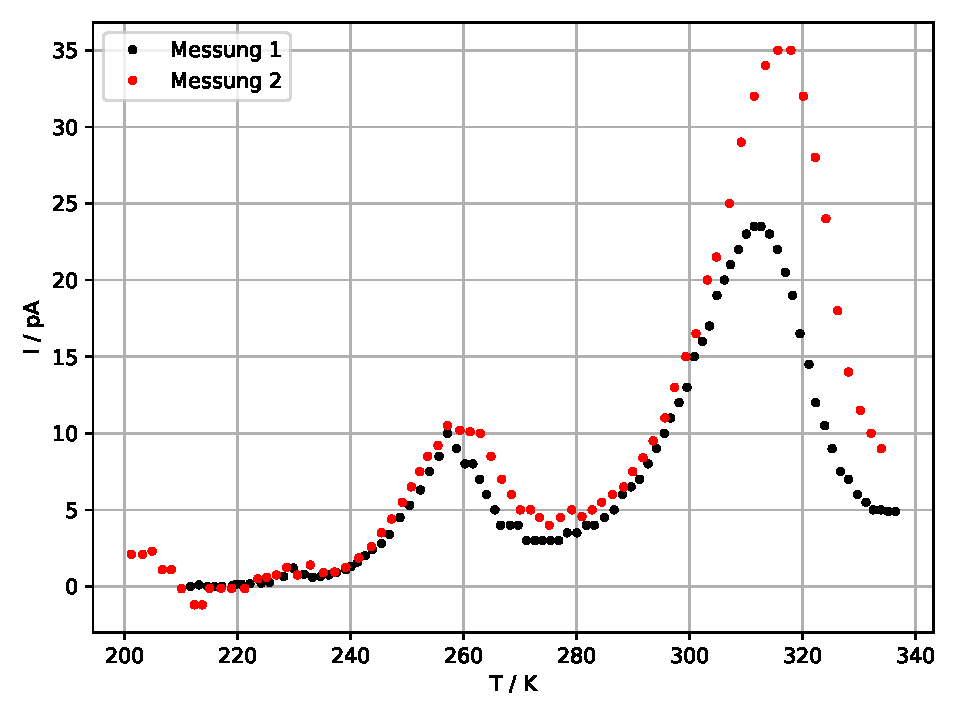
\includegraphics{build/plot.pdf}
  \caption{Die aufgenommenen Messwerte. Bei Messung 1 wird eine Heizrate von $b = \SI{1.5}{\celsius\per\minute}$ erzielt, 
  bei Messung 2 soll $b = \SI{2}{\celsius\per\minute}$ betragen.}
  \label{fig:T_I_plot_beide_Messung}
\end{figure} % OK, Heizrate mit Kelvin angeben ?

\begin{figure}
  \centering
  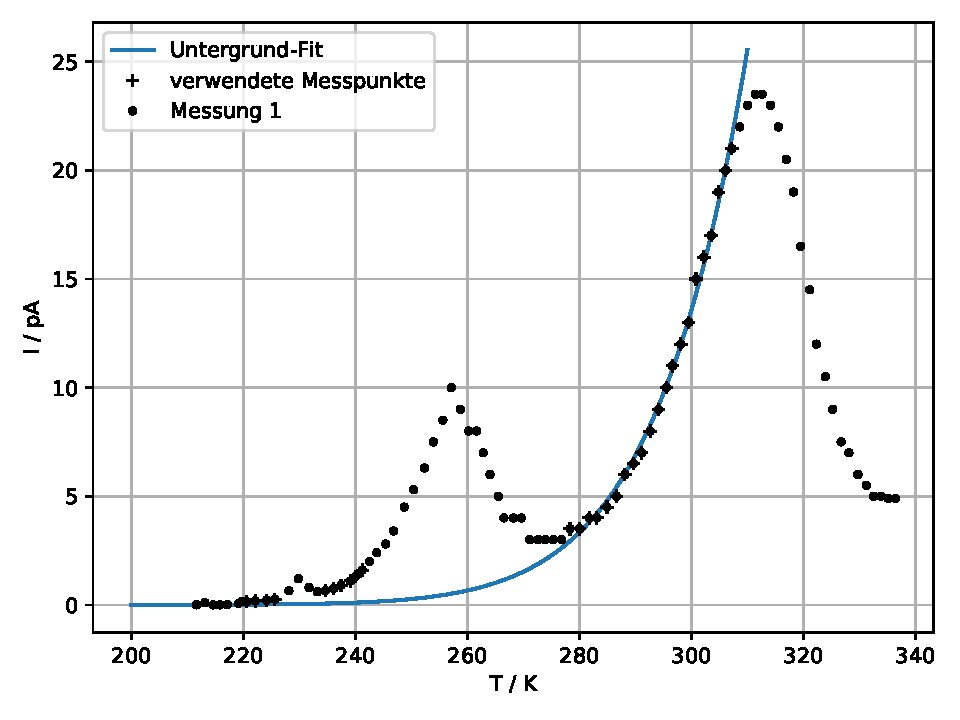
\includegraphics{build/untergrund_1.pdf}
  \caption{Die gefittete Untergrundfunktion mit der Form einer e-Funktion.
   Die Messwerte, die den Anstieg des zweiten Maximums bilden, werden für den Fit verwendet.}
  \label{fig:T_I_plot_1_Untergrund}
\end{figure} % OK

\begin{figure}
  \centering
  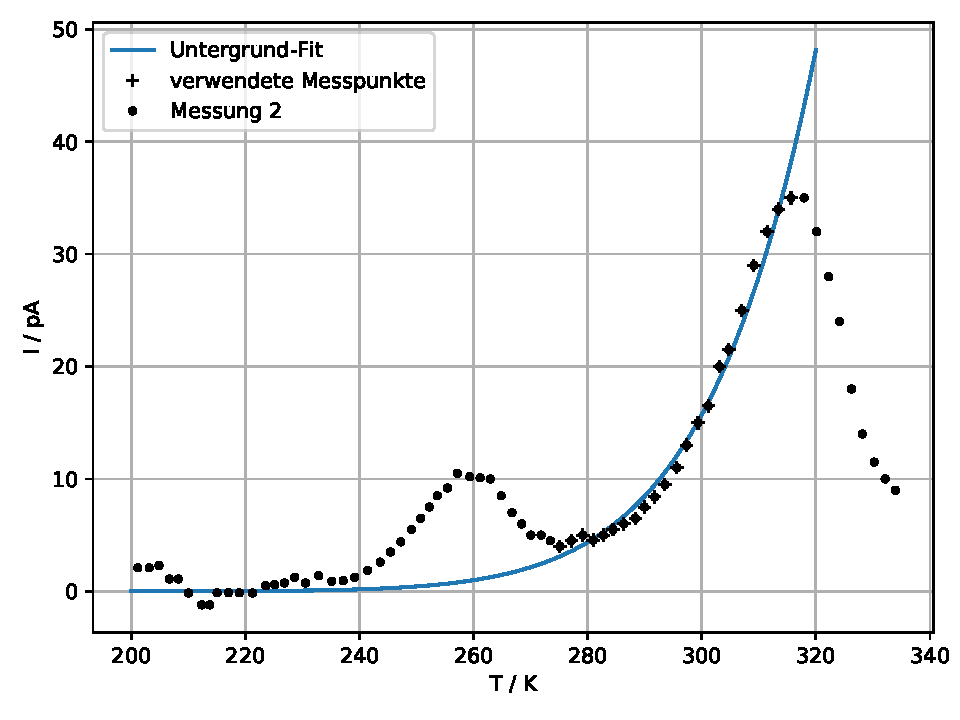
\includegraphics{build/untergrund_2.pdf}
  \caption{Die gefittete Untergrundfunktion mit der Form einer e-Funktion.
  Die Messwerte, die den Anstieg des zweiten Maximums bilden, werden für den Fit verwendet.}
  \label{fig:T_I_plot_2_Untergrund}
\end{figure} % OK, vielleicht beide Untergrund Fits in ein figure, weil beide gleiche bescheibung


\subsection{Heizrate bzw. erste Methode}

Die aufgenommenen Messwerte können auch in ein Zeit-Temperatur Diagramm dargestellt werden.
Dieses ist in \autoref{fig:t_T_plot} zu sehen.
Um die Heizrate der jeweiligen Messung zu bestimmen, wird eine lineare Ausgleichsrechnung durhgeführt.
Die zu fittende Funktion hat die Form
\begin{equation*}
  T(t) = b * t + T_0 \, .
\end{equation*}
Es ergibt sich für die erste Messung:
\begin{align*}
  b = 1.46 \pm  0.0037 &&  T_0 = 210.92 \pm 0.1885\\
\end{align*}
und für die zweite Messung:
\begin{align*}
  b =  1.87 \pm 0.0049  &&  T_0 = 198.95 \pm  0.2027 \, . \\
\end{align*}
Die beiden Messungen sowie ihre jeweiligen Ausgleichsgeraden sind in \autoref{fig:t_T_plot_1_Ausgleich} und \autoref{fig:t_T_plot_2_Ausgleich} zu sehen.

\begin{figure}
  \centering
  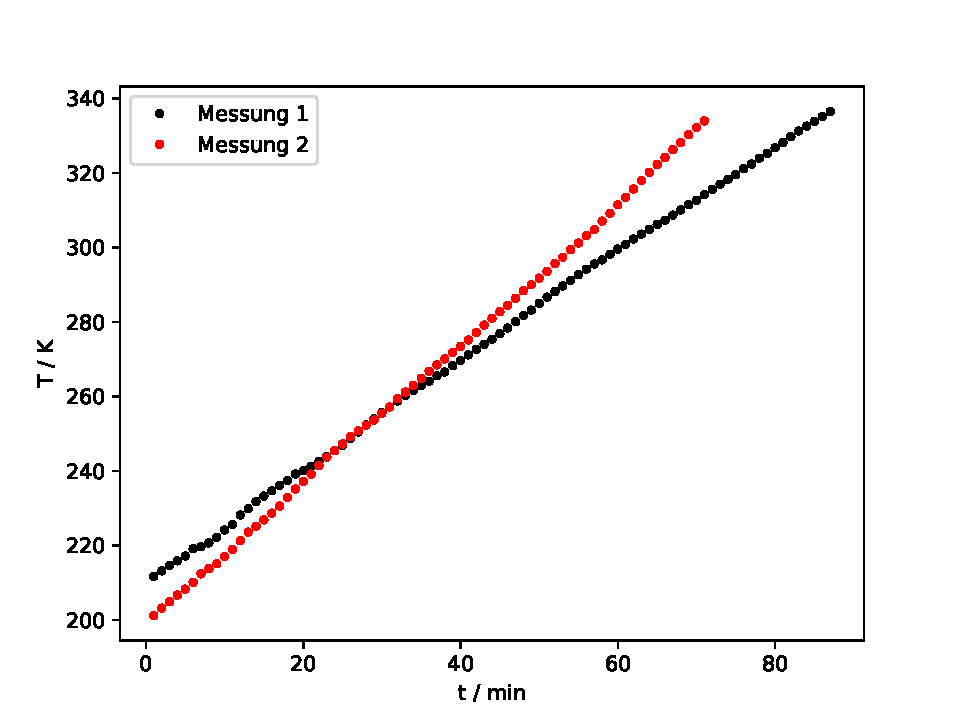
\includegraphics{build/zeit_temp.pdf}
  \caption{Die aufgenommenen Messwerte. Bei Messung 1 wird eine Heizrate von $b = \SI{1.5}{\celsius\per\minute}$ erzielt, 
  bei Messung 2 soll $b = \SI{2}{\celsius\per\minute}$ betragen.}
  \label{fig:t_T_plot}
\end{figure} % OK, eig könnte man beschreibung so lassen bzw. wat soll man sonst da schreiben

\begin{figure}
  \centering
  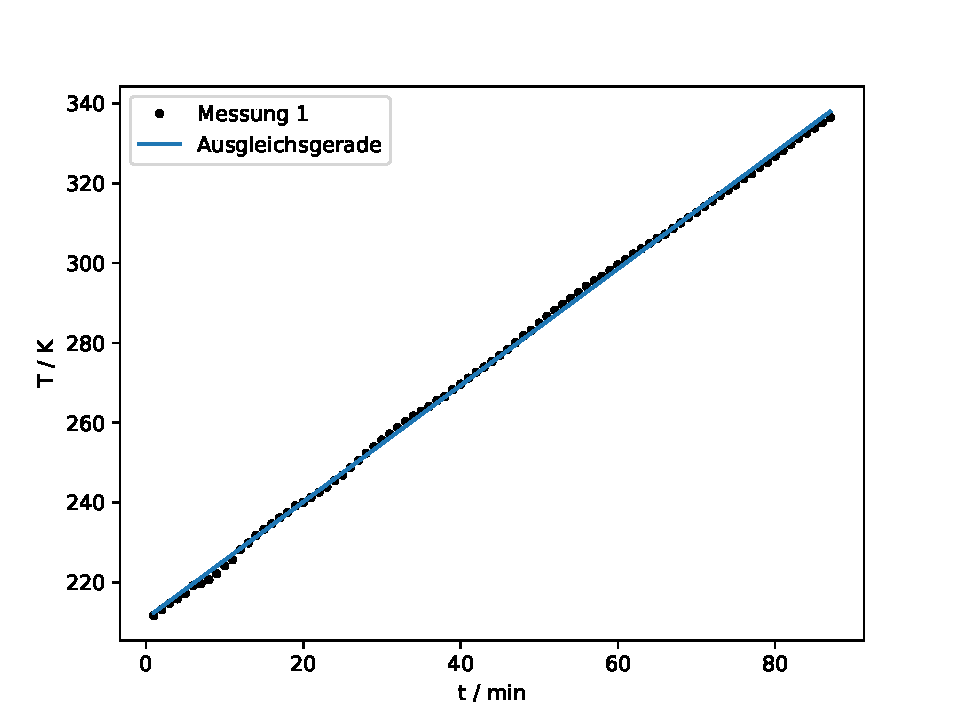
\includegraphics{build/zeit_temp_fit_1.pdf}
  \caption{Die aufgenommenen Messwerte der Messung 1 und der dazugehörige Fit. Bei Messung 1 wird eine Heizrate von $b = \SI{1.5}{\celsius\per\minute}$ erzielt.
    Durch die Ausgleichsrechnung ergibt sich fü $b = \SI{}{\celsius\per\minute}$.}
  \label{fig:t_T_plot_1_Ausgleich}
\end{figure} % OK, vielleicht auch ermittelte Heizrate hier rein schreiben?

\begin{figure}
  \centering
  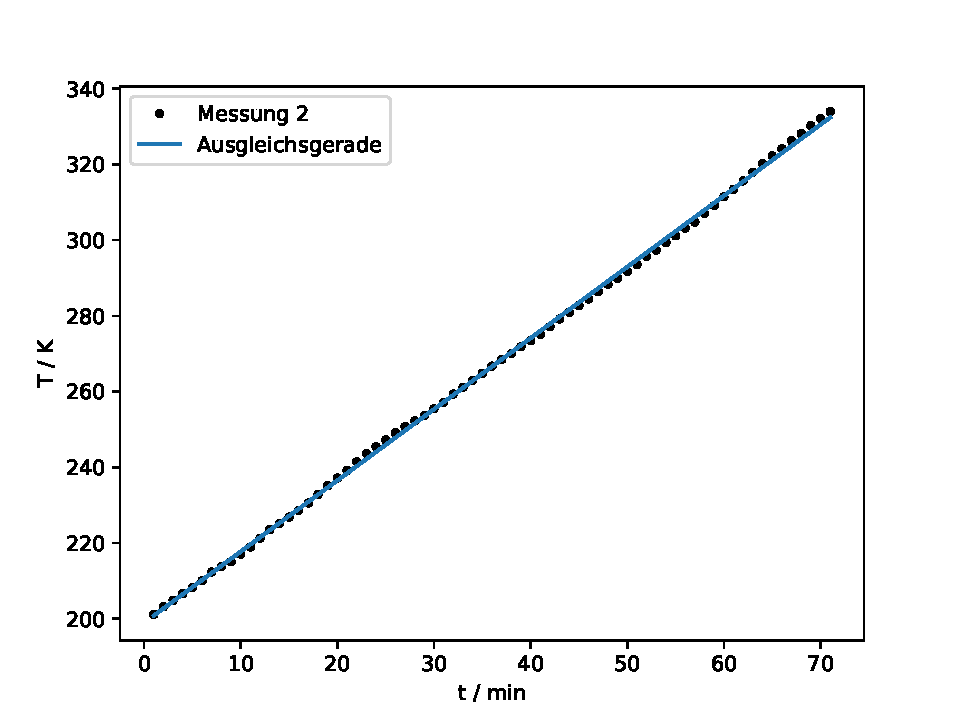
\includegraphics{build/zeit_temp_fit_2.pdf}
  \caption{Die aufgenommenen Messwerte der Messung 2 und der dazugehörige Fit. Bei Messung 2 wird eine Heizrate von $b = \SI{2}{\celsius\per\minute}$ erzielt.
  Durch die Ausgleichsrechnung ergibt sich fü $b = \SI{}{\celsius\per\minute}$.}
  \label{fig:t_T_plot_2_Ausgleich} 
\end{figure} % OK, vielleicht auch ermittelte Heizrate hier rein schreiben?

Zur Bestimmung der Aktivierungsenergie mithilfe des Maximums werden die Messwerte zunächst in eine andere darstellungsweise gebracht.
Nach THEORIE wird der Logarithmus des Depolarisationsstrom gebildet und gegen die Inverse Temperatur abgebildet.
Die jeweiligen Diagramme sind in \autoref{fig:log_I_1_durch_T_Messung_1} und \autoref{fig:log_I_1_durch_T_Messung 2} zu finden.
Mithilfe von THEORIE wird eine Ausgleichsrechnung durchgeführt.
Die zu fittende Funktion hat dabei die Form
\begin{equation*}
  \ln{I(T)} = c - m \cdot \frac{1}{T} \, .
\end{equation*}
Die ermittelten Werte sind für Messung 1:
\begin{align*}
  c = 28.03 \pm  0.61 && m = -6630.94 \ pm 145.12  \,  \\
\end{align*}
und für Messung 2:
\begin{align*}
  c = 23.01 \pm  1.67 && m = -5337.54 \ pm 403.39  \, . \\
\end{align*}
Die Ausgleichsgeraden sind ebenfalls in \autoref{fig:log_I_1_durch_T_Messung_1} und \autoref{fig:log_I_1_durch_T_Messung 2} zu finden.

\begin{figure}
  \centering
  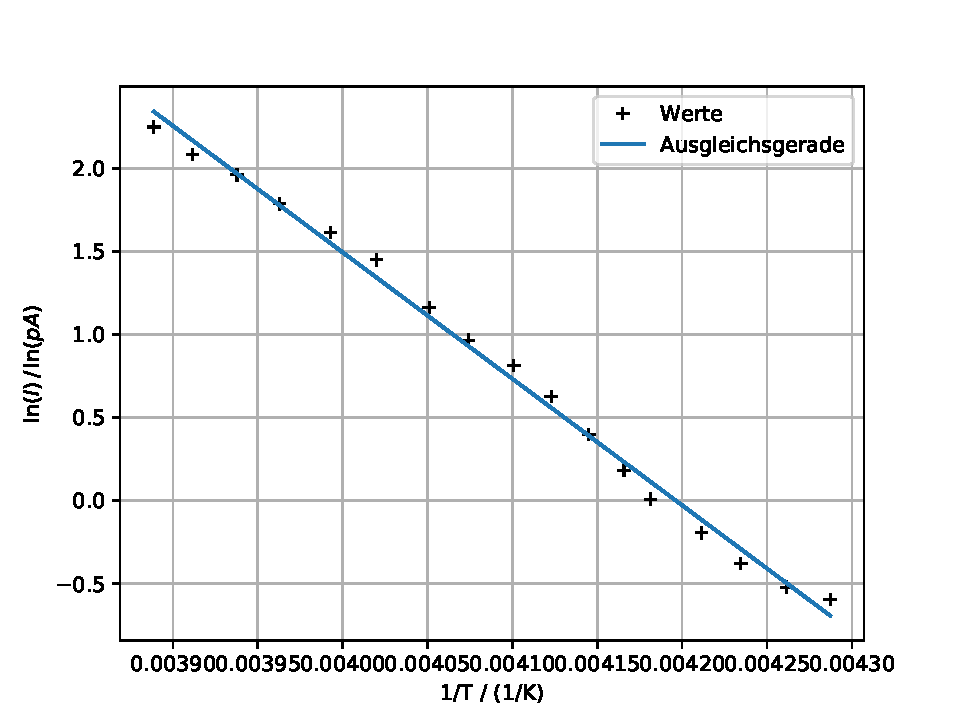
\includegraphics{build/log(I)_1durchT_1.pdf}
  \caption{$\log{I} gegen \frac{1}{T}$ aufgetragen.}
  \label{fig:log_I_1_durch_T_Messung_1}
\end{figure} % OK, beschreibung?

\begin{figure}
  \centering
  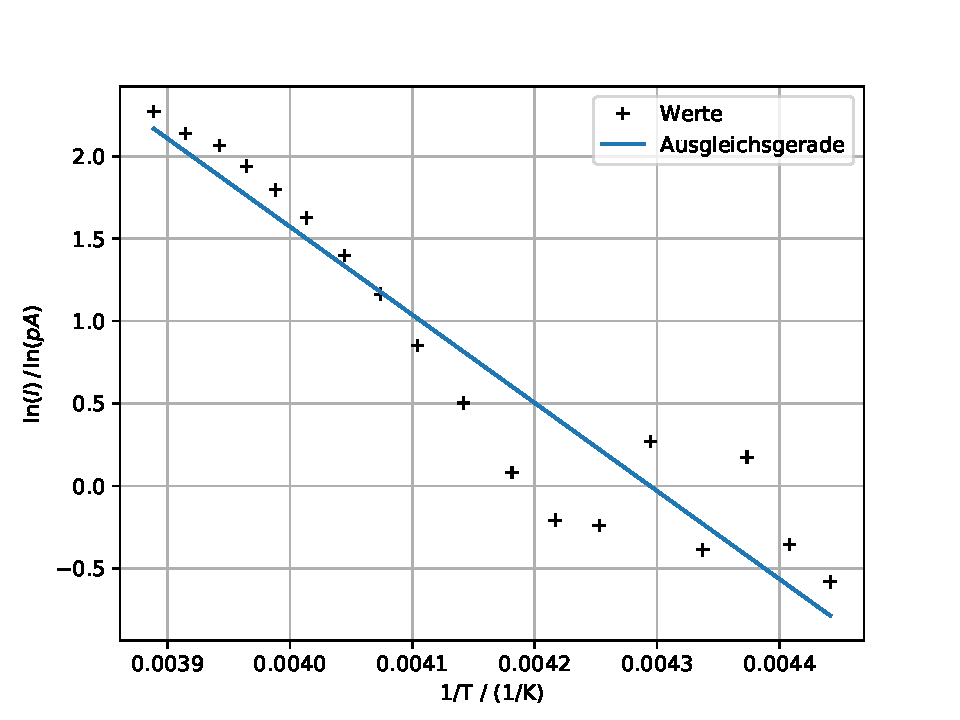
\includegraphics{build/log(I)_1durchT_2.pdf}
  \caption{was sagt uns das? genau. gar nichts}
  \label{fig:log_I_1_durch_T_Messung 2}
\end{figure} % Ok, Beschreibung?
% also hier hab ich den untergrund noch nicht abgezogen idk, im plot.py hab ich jetzt ausprobiert aber sind mies aus ka, bzw idk wie das aussehen soll,
% ok hab das jetzt gemacht idk 
Aus THEORIE ergibt sich dann für die jeweilige Aktivierungsenergie $W$
\begin{align}
  W = -k_\text{B} \cdot m \\
  W_1 = -6630.94 \ pm 145.12 \cdot -k_\text{B} \\
  W_2 = -5337.54 \ pm 403.39 \cdot -k_\text{B}\\
\end{align}

\subsection{Methode 2}
Der korrigierte Stromverlauf wird nun betrachtet.
Dieser ist für beide Messungen in \autoref{fig:I_T_korrigiert_1} und \autoref{fig:I_T_korrigiert_2} zu finden.

\begin{figure}
  \centering
  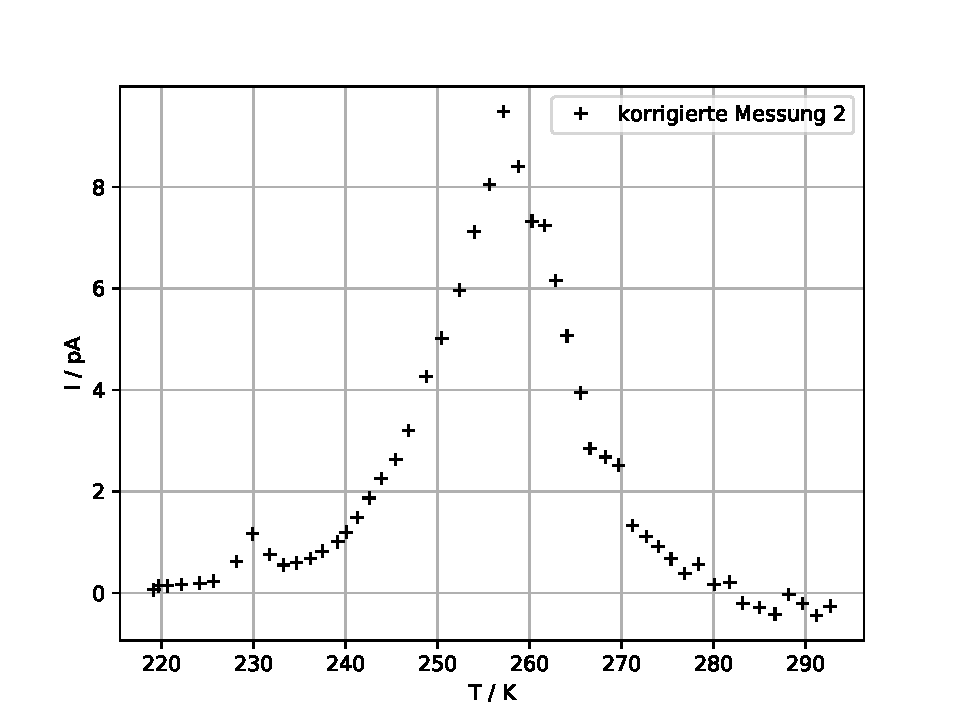
\includegraphics{build/korrigierte_werte_1.pdf}
  \caption{Korrigierten Messwerte der Messung 1}
  \label{fig:I_T_korrigiert_1}
\end{figure} % OK idk

\begin{figure}
  \centering
  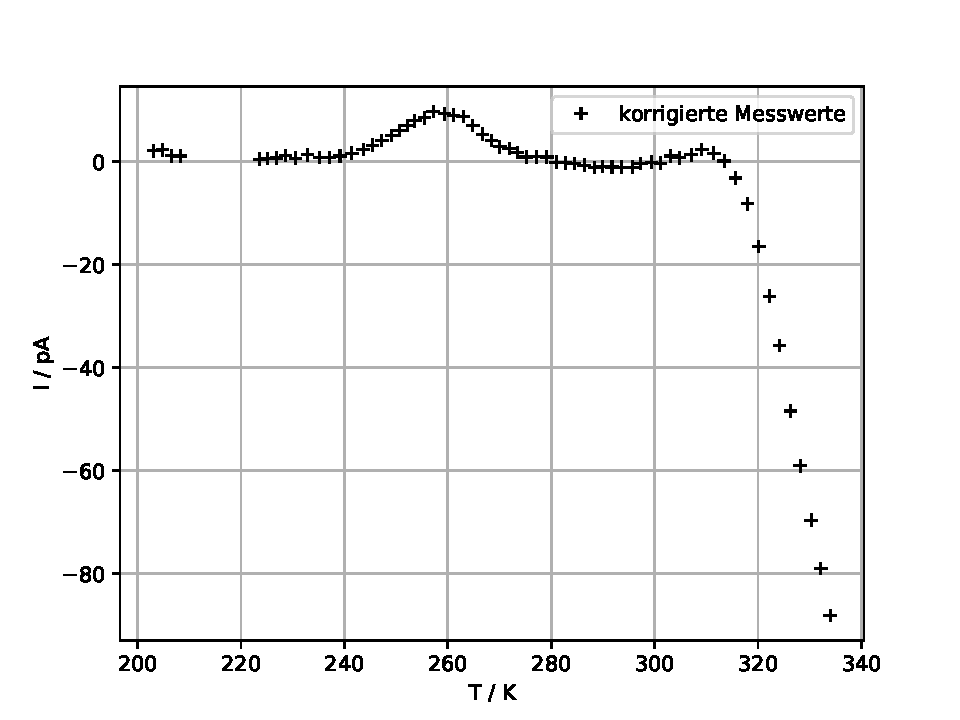
\includegraphics{build/korrigierte_werte_2.pdf}
  \caption{Korrigierten Messwerte der Messung 2}
  \label{fig:I_T_korrigiert_2}
\end{figure} % OK idk